%===============================================================
\section{Motivation}

\subsection{State of World}

The fundamental challenge of JS engine fuzzing can be summed up by the observation that,
while we know the comeplte source and specification of our target source and exploitation language, respectively,
the number of degrees of freedom in such an envrionment is much too large to allow for a direct, instantaneous
identification of all vulnerabilities. This observation is reflected in the multitude of architectures and
approaches in today's JS engine fuzzers.

The space of today's JavaScript engine fuzzers can best be understood
as two mutually non-exclusive architectures: generative and mutational.
\vspace{-1em}%

\p{Generative fuzzers} posit new test cases 
(i) from scratch based on a predefined grammar, e.g., DOMato\cite{domato} and Dharama\cite{dharma}, or
(ii) by constructing them from synthesizable code blocks, e.g., CodeAlchemist\cite{codealchemist_2019} and Fuzzilli\cite{saelo_thesis}.

\p{Mutational fuzzers} posit new test cases using segments either learned from seed-based mutations
or borrowed from other corpora programs, e.g., Skyfire\cite{skyfire_2017}, Fuzzilli\cite{saelo_thesis},
Nautilus\cite{nautilus_2019}, Superion\cite{superion_2019}, and DIE\cite{die_2020}.

%-----------------------------------------
\subsection{JSC Speculative Type [Confusion]}

%<Short paragraph on the focus of JIT compilers and type speculation>
One of the more prominant observed vulnerabilty classes, type confusion vulnerabilities often require a complex 
control and/or data flow within the phases of an optimization pipeline. During a given optimization phase,
JavaScript code is profiled, variable types are speculated, and optimized bytecode is produced\footnotemark.
\footnotetext{Poor type speculation results in execution a priori; JSC defaults to unoptimized interpreter bytecode execution.}
A side-by-side view of JSC's speculative optimzation workflow and a standard C-based compiler's equivalent is
provided in Figure 2.

%As we've seen, there are too many components of the JS engine to cover -- following recent exploitation trends,
%we will focus our time (and this paper) on JavaScriptCore's two most attacked components: the \textbf{Data Flow Graph (DFG)}
%and \textbf{Faster Than Light (FTL)} JIT compiler.%

%<we attack these such that we can focus on attacking type speculation, ideally looking for OOB RW>
\begin{itemize}
  \item One of the goals of DFG is to optimize away redundant operations such as type checks
  \item Only a few operations can alter an object’s type
  \item If no such operation is encountered, it can be
  assumed that the object type will stay unchanged
  and a single type check will suffice to prove the type
  of a specific value until some potentially dangerous
  operation is encountered
  \item Operations which may invoke arbitrary JavaScript are dangerous
  \item The arbitrary JavaScript may execute any operation, including things that may mutate an object’s type
  \item Important to model which operations may or may not do this in order to invalidate previously proven types
  \item We may cause arbitrary type confusions by mutating object types
\end{itemize}


%A high-level perspective of this compilation pipeline is presented in \textit{Figure 3}
%\begin{figure}[h]
%  \begin{center}
%    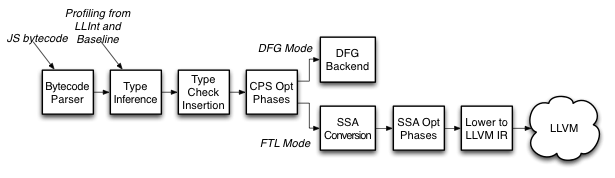
\includegraphics[width=0.5\textwidth]{img/ftl-pipeline}
%    \caption{The JavaScriptCore DFG/FTL JIT pipeline.}
%  \end{center}
%\end{figure}\vspace{-1.5em}

%-----------------------------------------
\subsection{WebAssembly}


\begin{itemize}
    \item WASM growing in popularity, in general
    \item Research into WASM-based fuzzing of JS engines underway, but not much novel research published
        %<opportunistic looking state of it's current research (no one is really fuzzing this)>
    \item WASM code is not JIT'd, thus it utilizes a different pipeline for execution, one that will not affect out primary research
\end{itemize}
%
